\chapter{Evaluation}
\label{chap:eval}

Our sampling data for testing our application were especially highly textured images of sculptures.
For detailed testing we have chosen two pairs of images shown in Figure \ref{fig:input_samples} taken with the Sony  ST27i device.
These data seemed to by ideal for testing while there was detected large number of good features such as corners, edges or other features that can be easily detected.

\begin{figure}[H]
\centering

\begin{subfigure}[b]{0.45\textwidth}
\centering
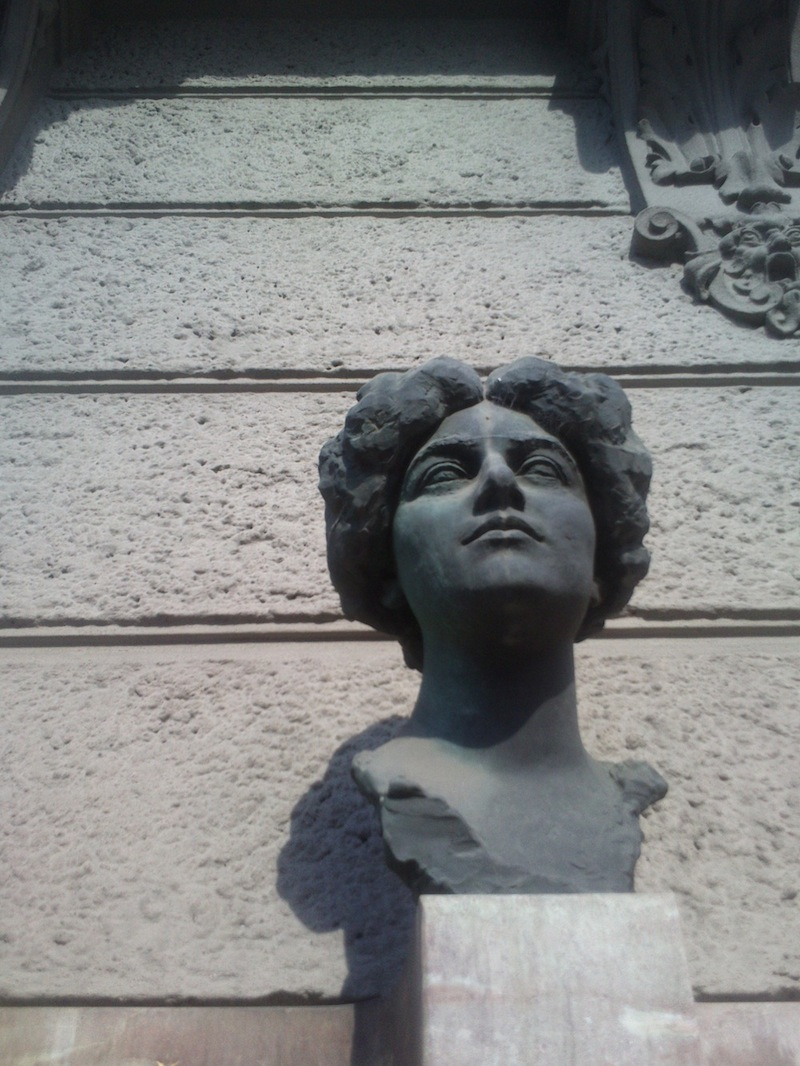
\includegraphics[width=6.0cm]{img/ema_a.png}
\caption{The left image of a bust of Ema Destinová.} \label{0}
\end{subfigure}
\begin{subfigure}[b]{0.45\textwidth}
\centering
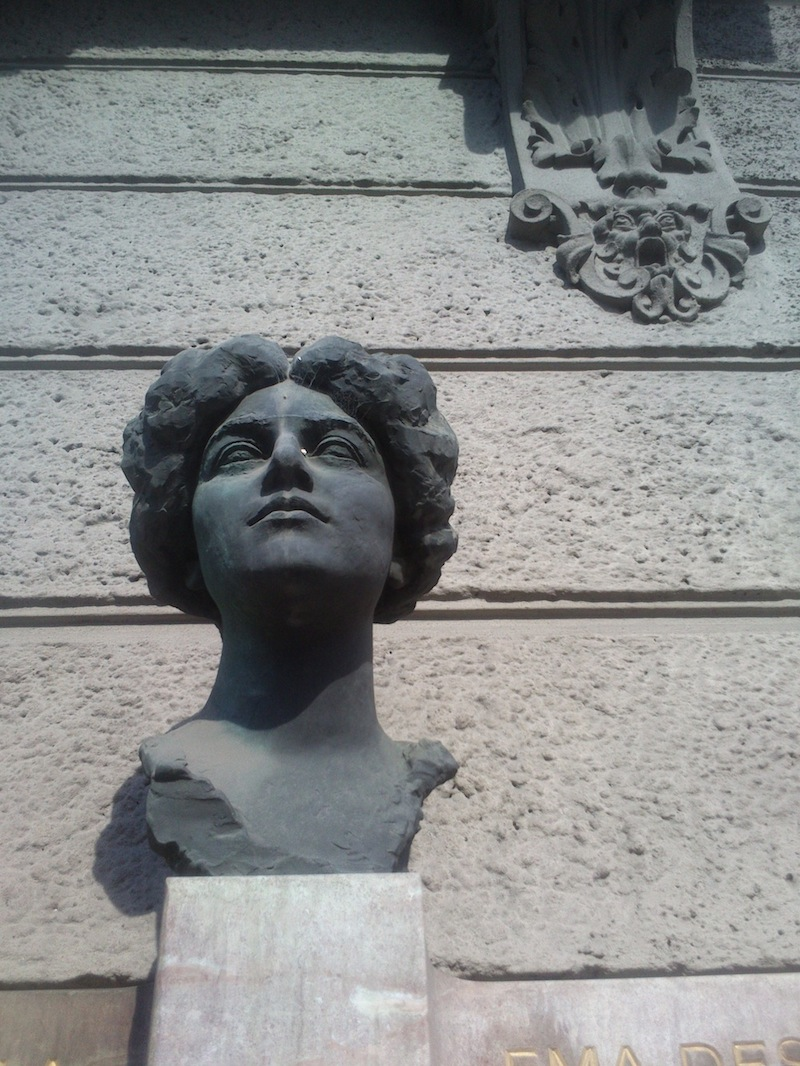
\includegraphics[width=6.0cm]{img/ema_b.png}
\caption{The right image of a bust of Ema Destinová.} \label{2}
\end{subfigure}
\begin{subfigure}[b]{0.45\textwidth}
\centering
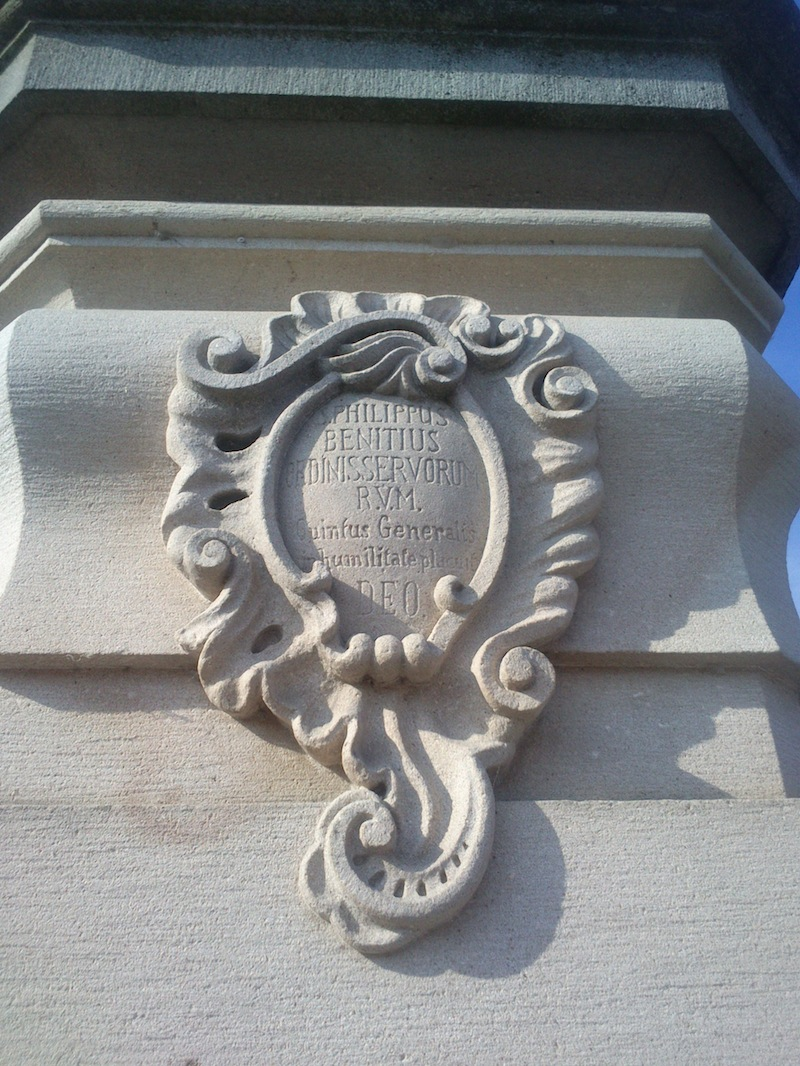
\includegraphics[width=6.0cm]{img/memorial_a.png}
\caption{The left image of a memorial.} \label{3}
\end{subfigure}
\begin{subfigure}[b]{0.45\textwidth}
\centering
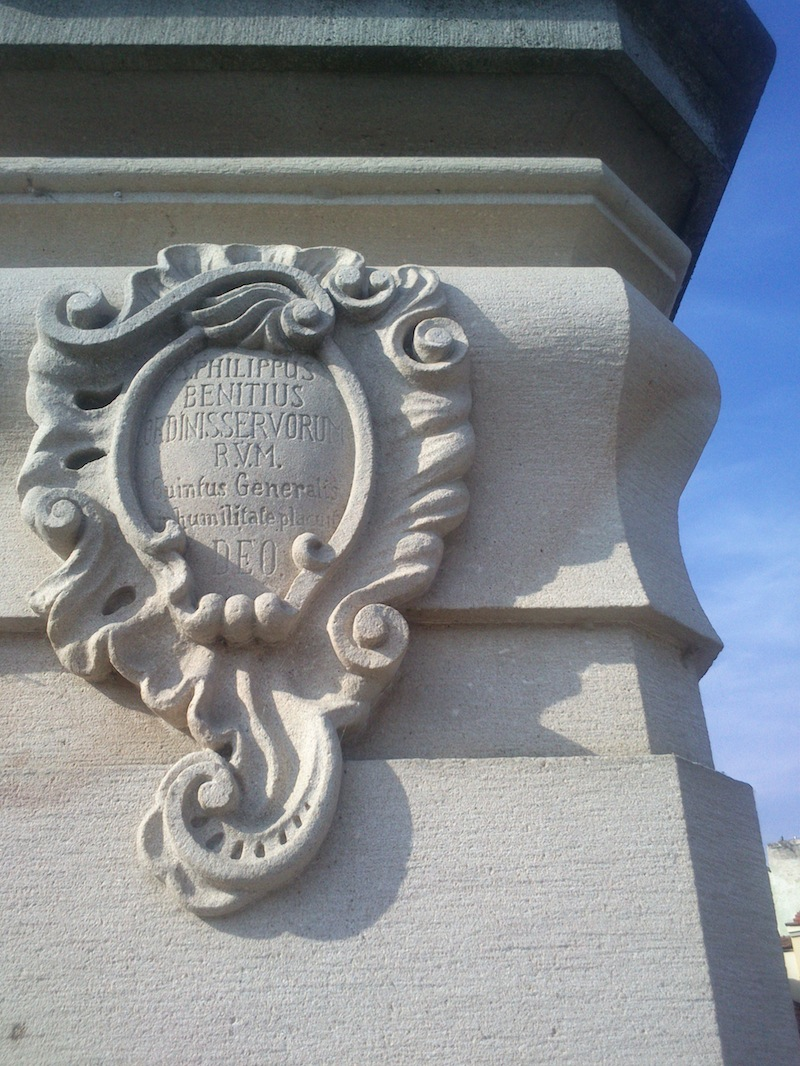
\includegraphics[width=6.0cm]{img/memorial_b.png}
\caption{The right image of a memorial.} \label{4}
\end{subfigure}

\caption[]{Examples of expecting pairs of the input images.} 
\label{fig:input_samples}
\end{figure}


\section{Results}
For our testing input data shown in Figure \ref{fig:input_samples} the results seem satisfying.
For this kind of input the SURF detector works properly.
It detects sufficient amount of keypoints and after filtering there remain enough good matches to get the information about the depth of some parts of the input images.

\begin{figure}[h]
\centerline{
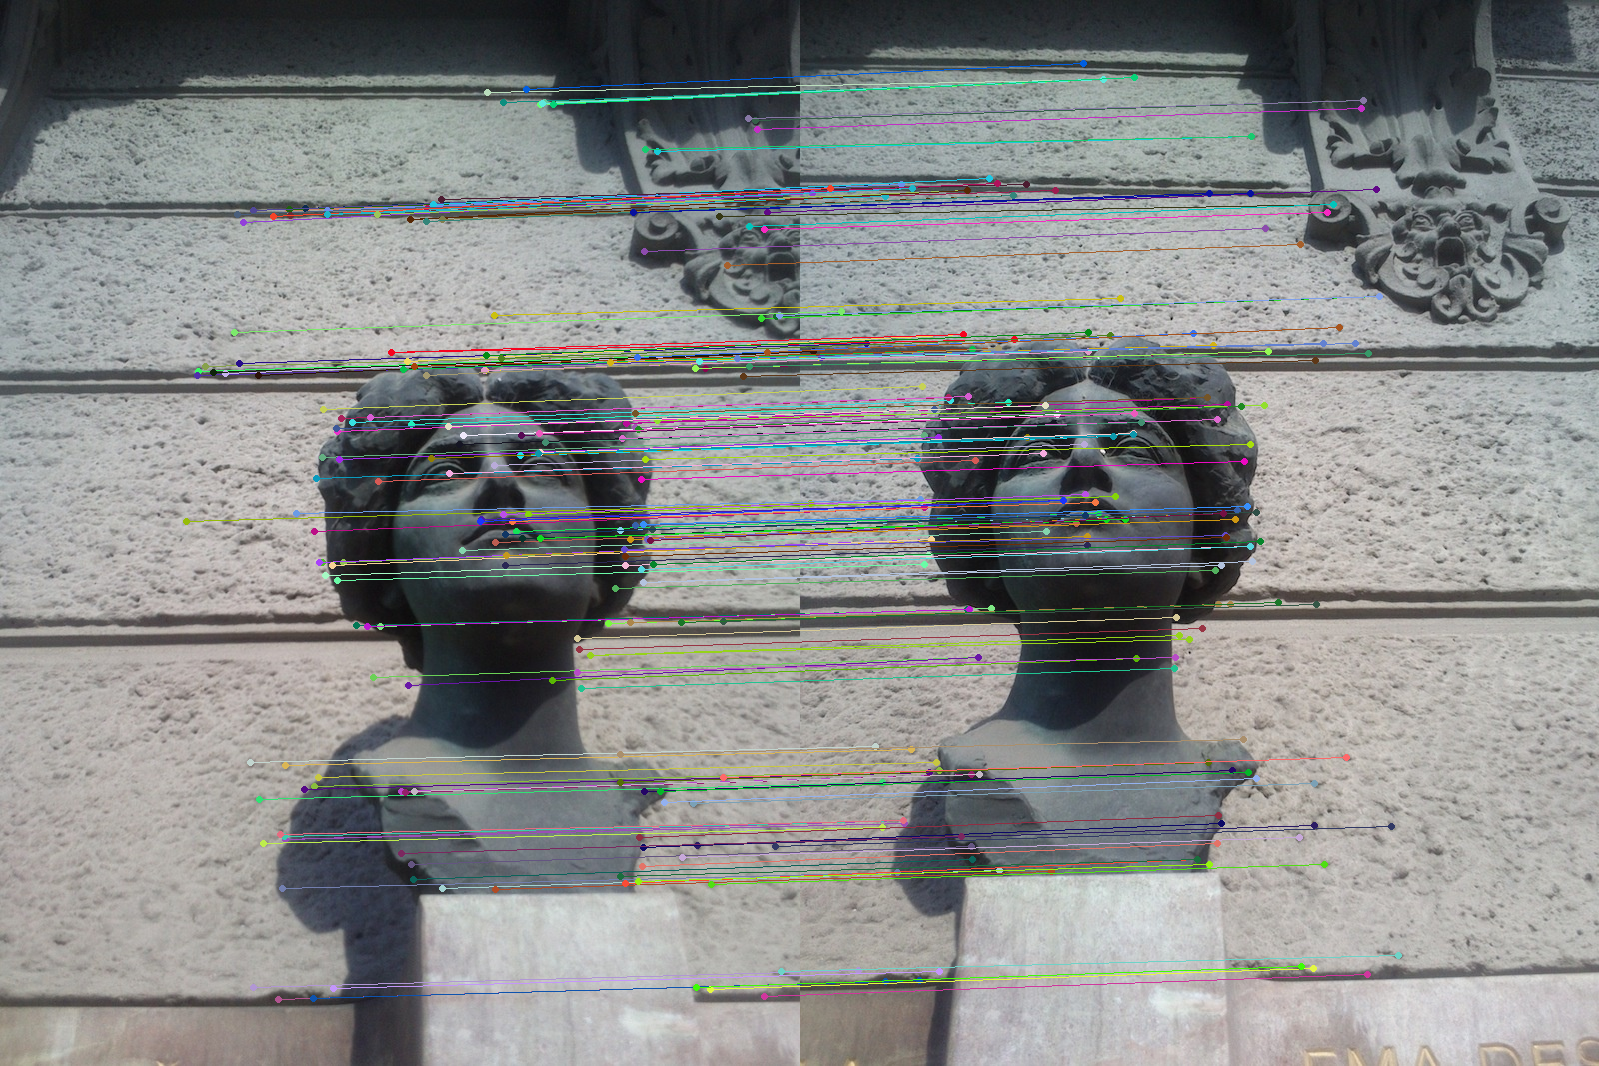
\includegraphics[width=12.0cm]{img/ema_matching.png}}
\centerline{
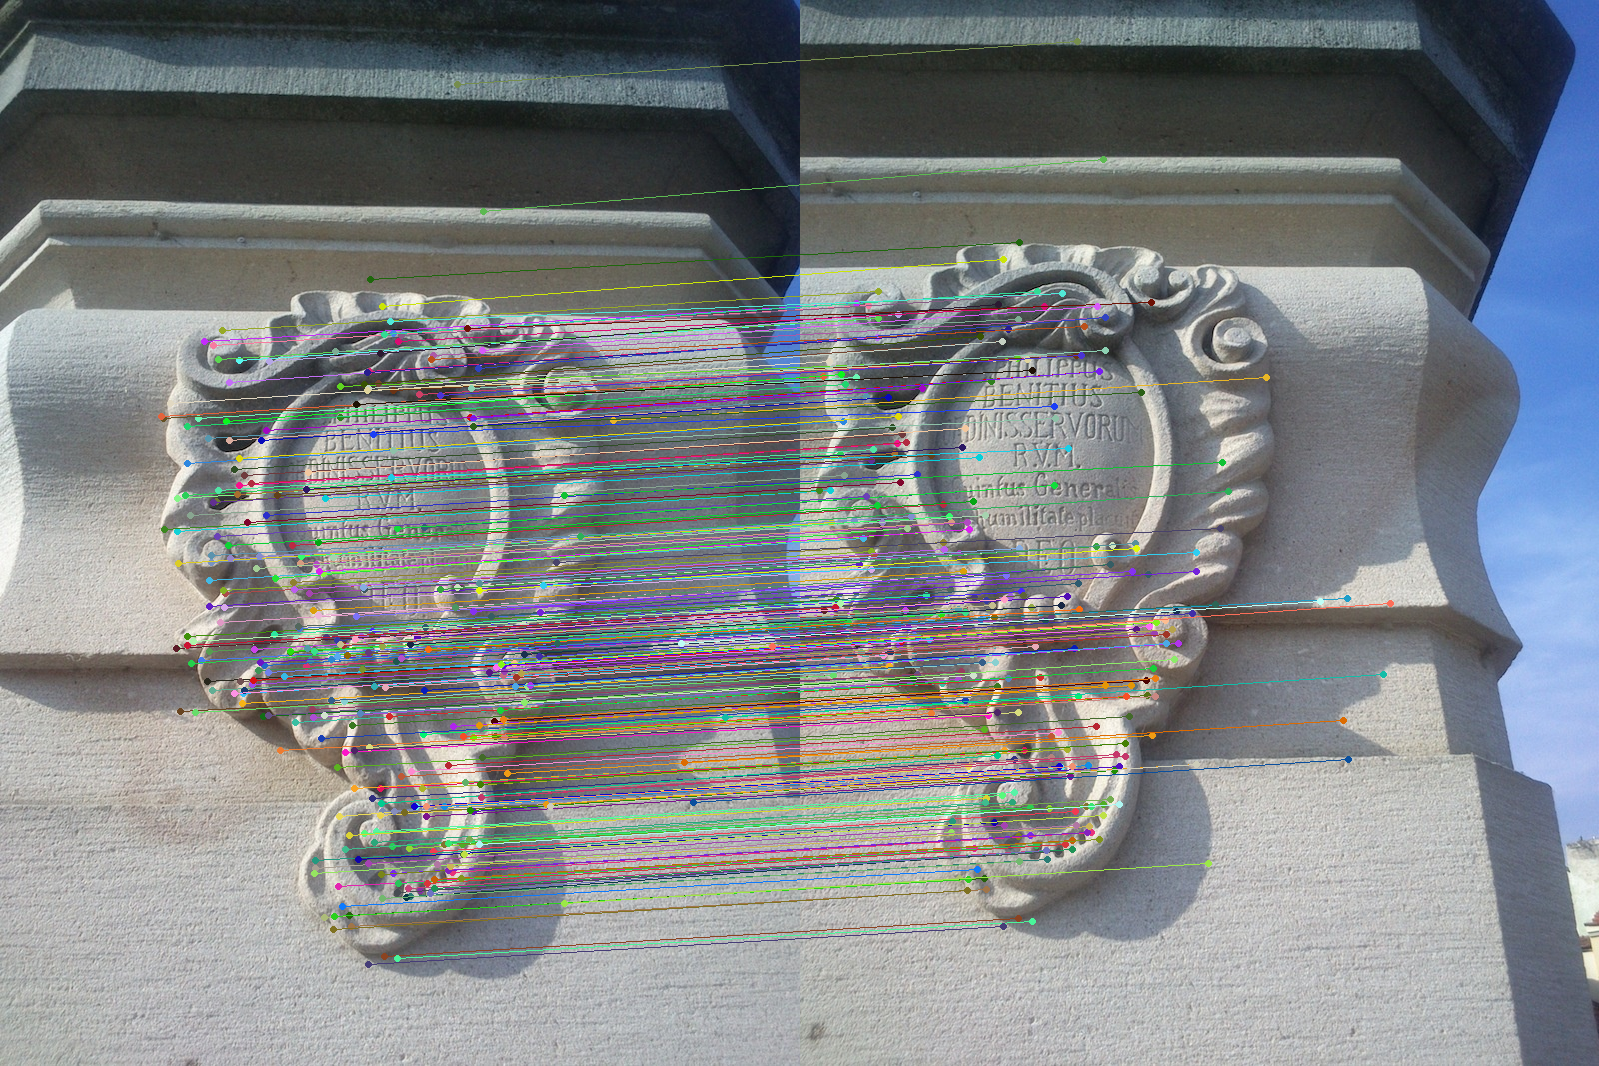
\includegraphics[width=12.0cm]{img/memorial_matching.png}}
\caption{The results of SURF matching.}
\label{fig:matching}
\end{figure}

For the pair of the images of a bust of Ema Destinová we get a 3D model shaping the head and a part of a wall in the background.
The second mentioned pair of input images gives us a result as an inclined plane in the angle of the memorial in the picture.
These results are comparable with the real appearance of the scenes.

\begin{figure}[h]
\centerline{
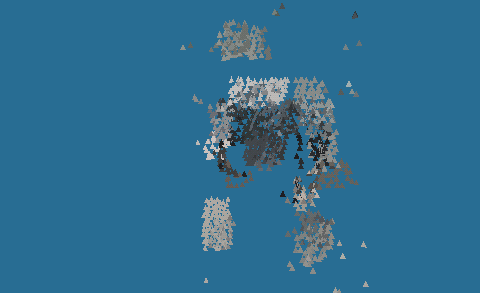
\includegraphics[width=6.5cm]{img/ema_3Dresult.png}
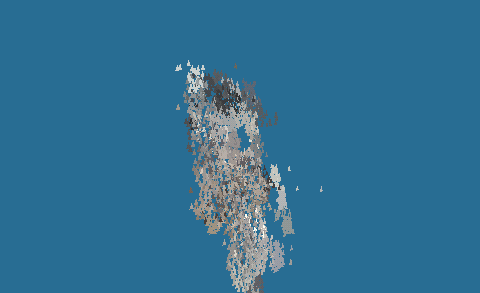
\includegraphics[width=6.5cm]{img/memorial_3Dresult.png}}
\caption{The output as a 3D model of disparity. The model of Ema Destinová sculpture (left) and of a memorial (right).}
\label{fig:outupt_samples}
\end{figure}

On the other hand for images with noise or images which are not highly textured, the result is usually a bunch of mismatches so the 3D model does not correspond with the reality.
An example of such input is shown in Figure \ref{fig:bad_example}.



\begin{figure}[h]
\centering

\begin{subfigure}[b]{0.45\textwidth}
\centering
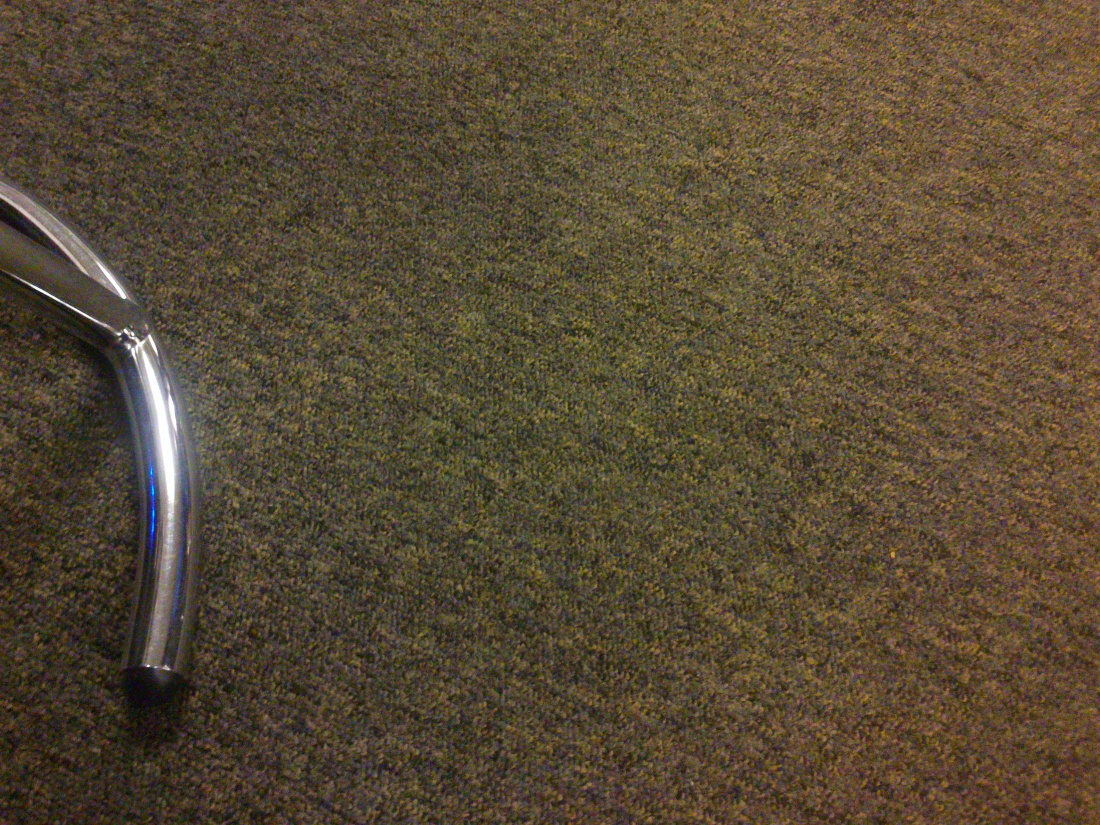
\includegraphics[width=4.5cm]{img/bad_input1.png}
\caption{The left image of the input image.} \label{x0}
\end{subfigure}
\begin{subfigure}[b]{0.45\textwidth}
\centering
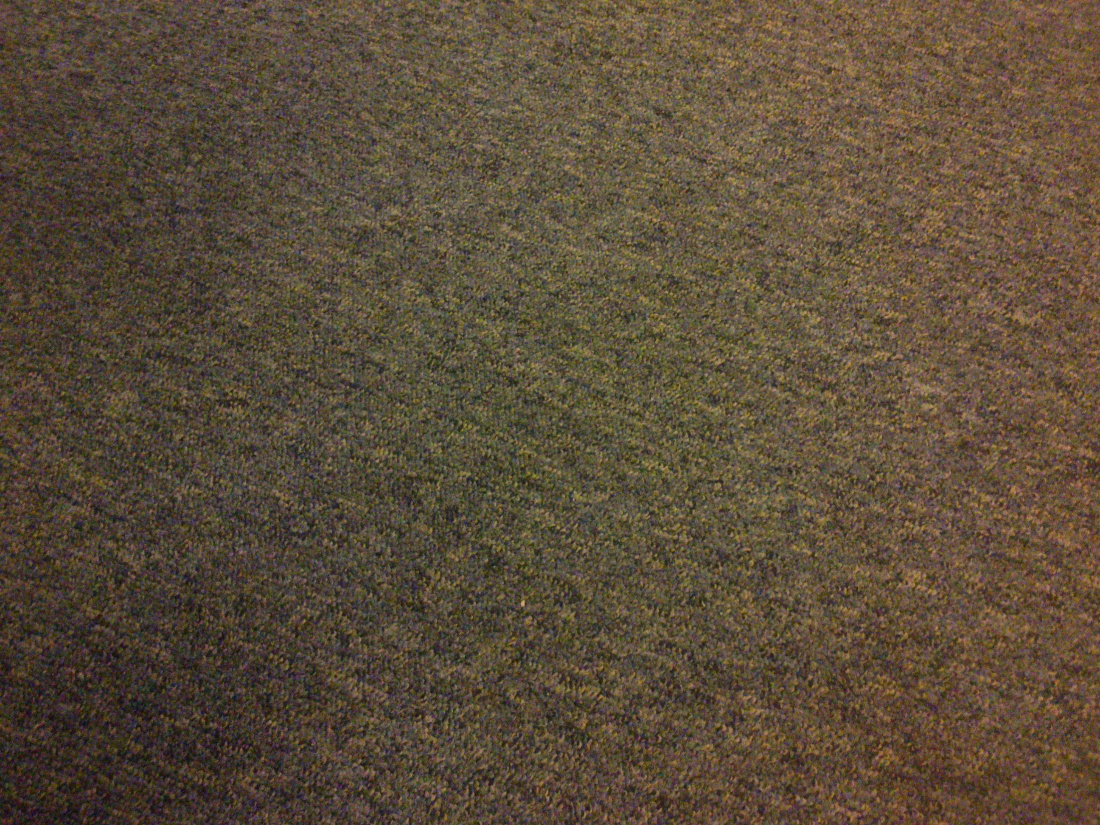
\includegraphics[width=4.5cm]{img/bad_input2}
\caption{The right image of the input image.} \label{x2}
\end{subfigure}
\begin{subfigure}[b]{0.45\textwidth}
\centering
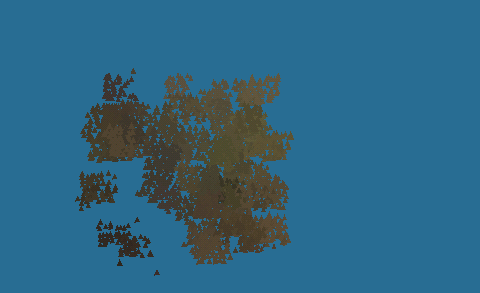
\includegraphics[width=5.0cm]{img/bad_result.png}
\caption{The result of the pair of images.} \label{x3}
\end{subfigure}

\caption[]{An example of a pair of images resulting in a nonrealistic model.} 
\label{fig:bad_example}
\end{figure}

When testing our application we have experimented with some parameters to get the best result.
In Figure \ref{fig:matching_comparison} we can see how was the result of matching affected when choosing different parameters for the second matching of SURF keypoints.
Each keypoint in the first image was matched with a keypoint in the estimated corresponding surrounding area in the second image in the shape of oriented rectangle computed according to the more accurate relative image position.
This oriented rectangle consists of two rectangles -- one exterior (60 $\times$ 120 pixels large) and smaller one localised in the middle of the previous one.
The corresponding keypoint was accepted only if it was located in the inner one.
In the first case, the size of the inner rectangle was set to 20\% of the width and 35\% of the height of the size of the larger rectangle.
The second image shows the result when the size was set to the 10\% of the width and 20\% of the height.
It was shown that the second case gives better results and we can see that there is less mismatches than in the first case.

\begin{figure}[H]
\centerline{
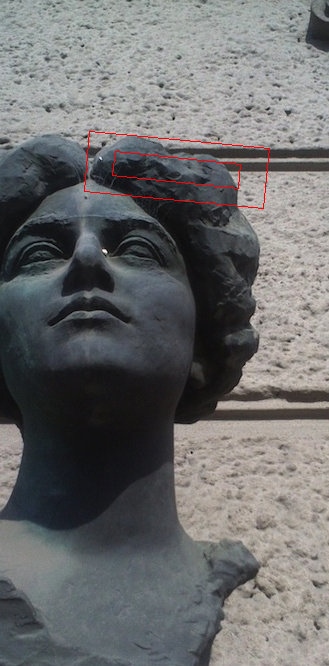
\includegraphics[width=4.0cm]{img/rectangle_w_02_h_035_croped.png}
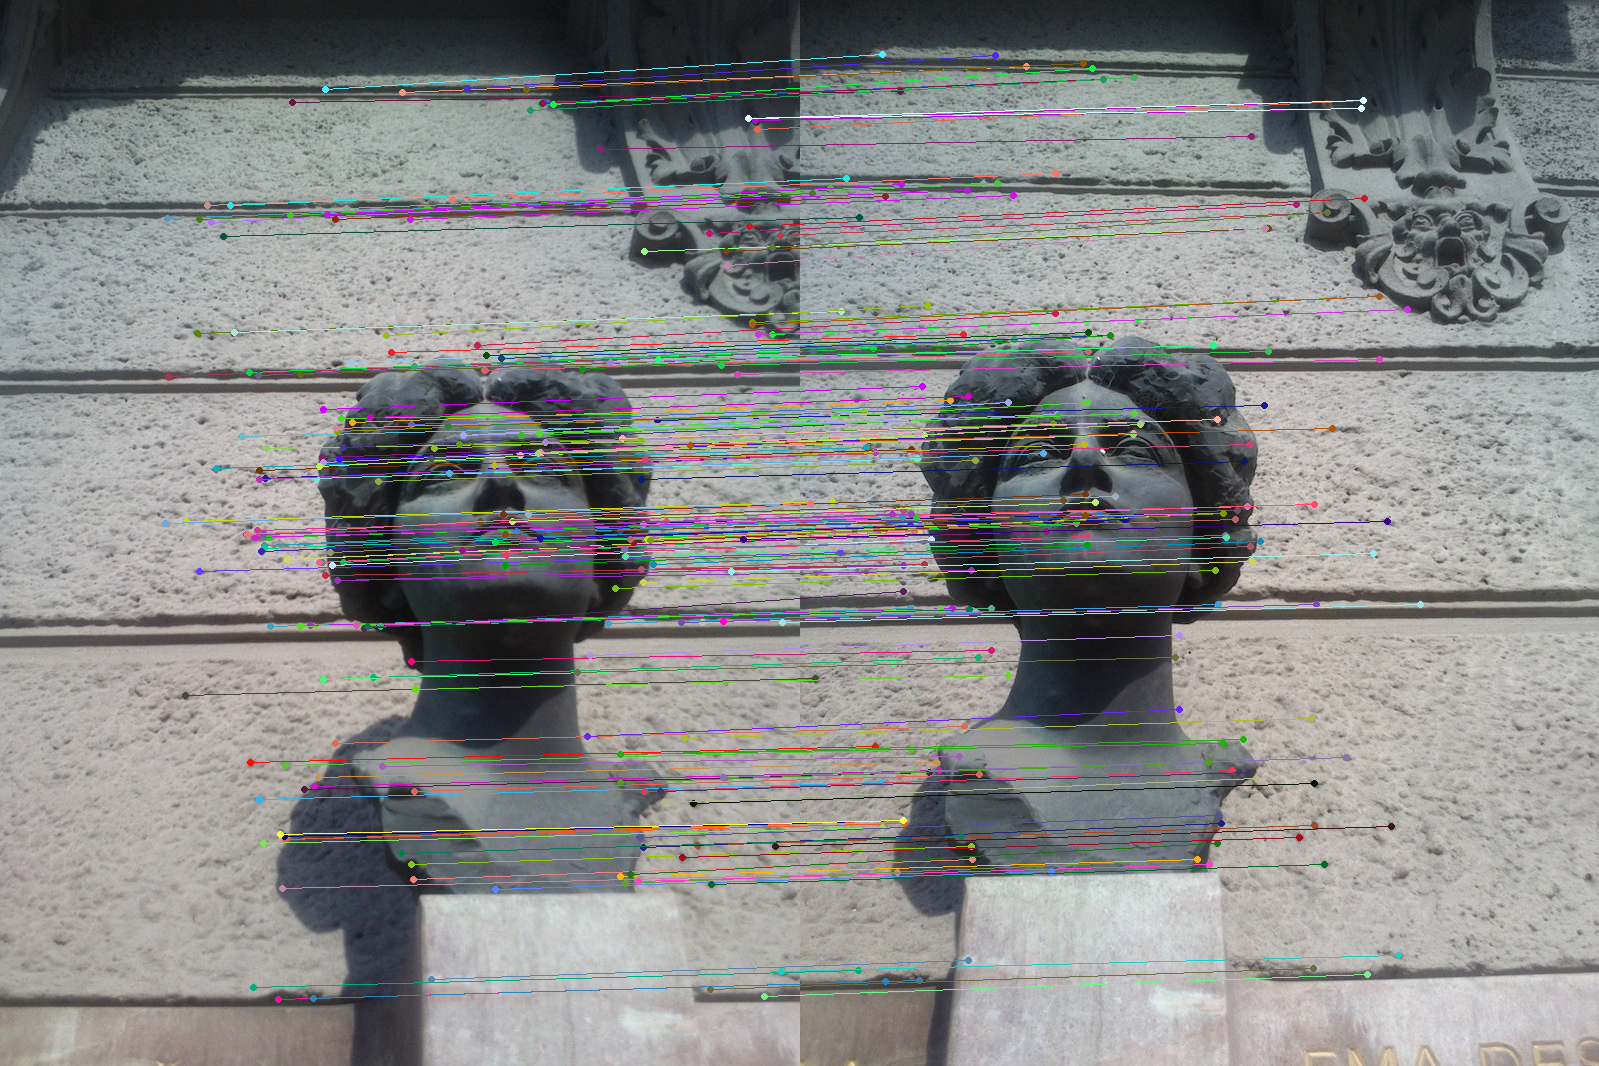
\includegraphics[width=12.1cm]{img/matching_w_02_h_035.png}}
\centerline{
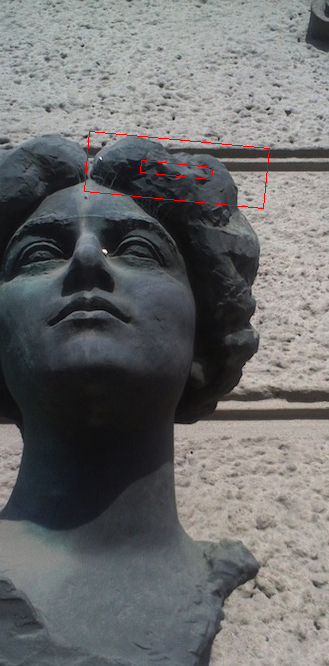
\includegraphics[width=4.0cm]{img/rectangle_w_01__h_02_croped.png}
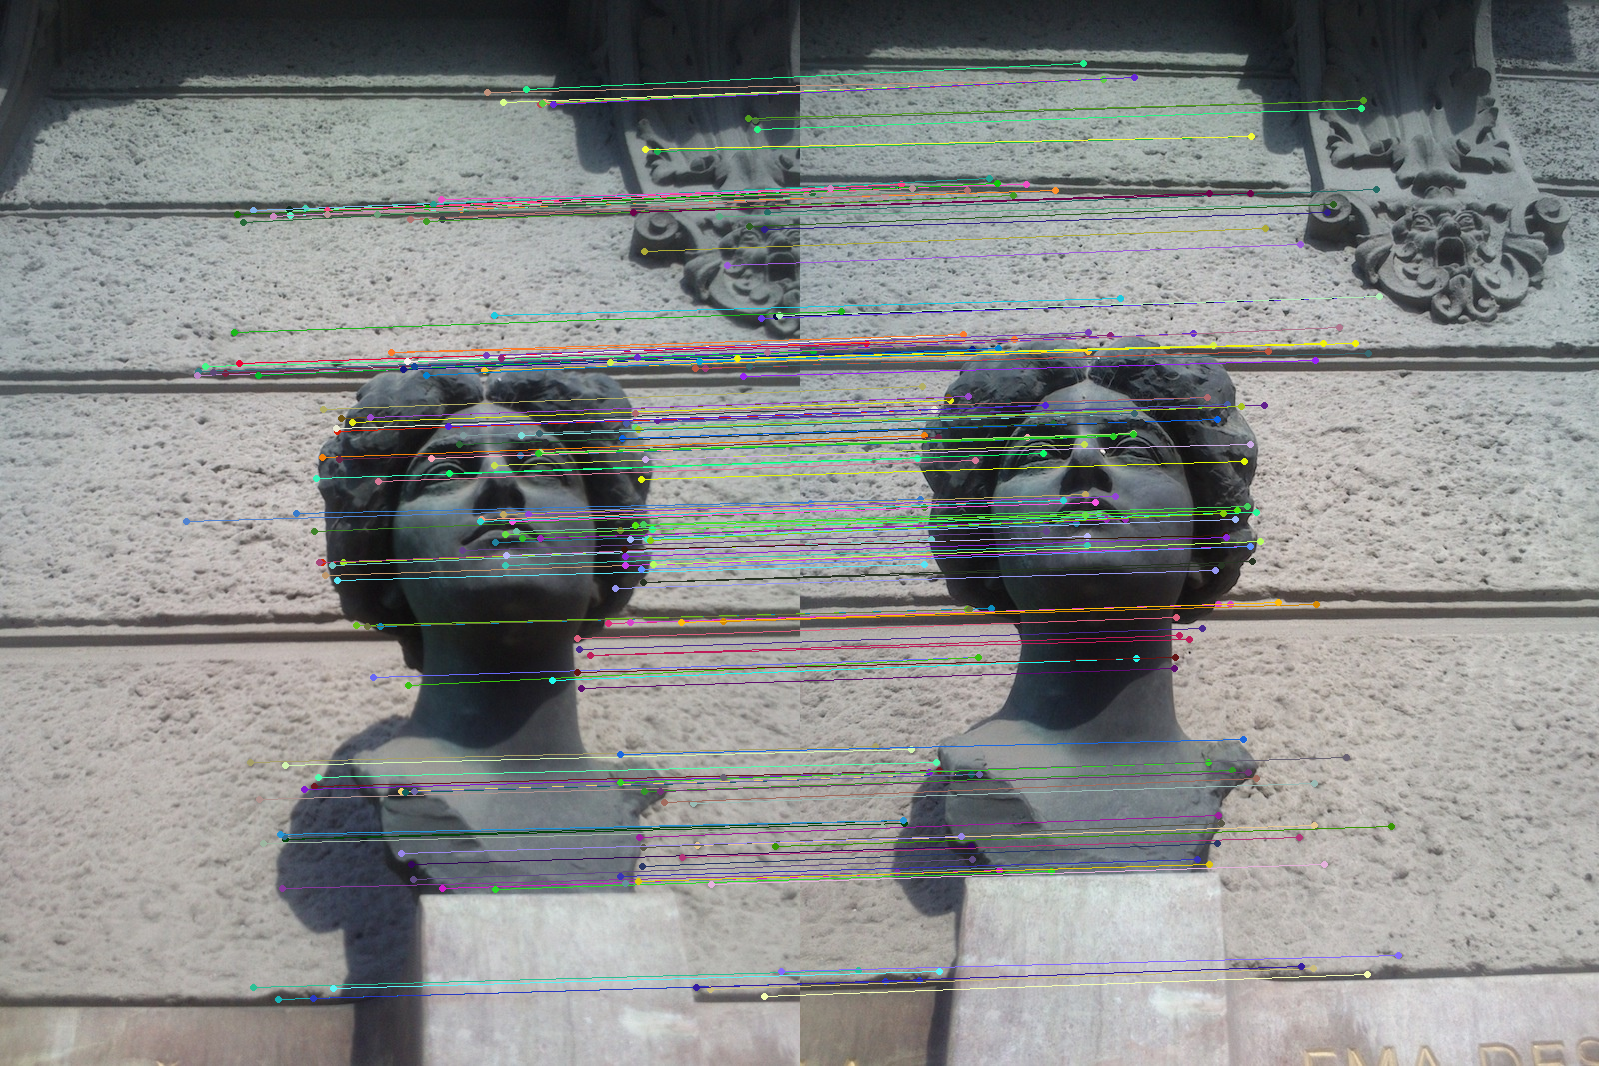
\includegraphics[width=12.1cm]{img/matching_w_01_h_02.png}}
\caption{Comparison of the result of matching with different sizes of the oriented rectangles. 
At the top left is a sample of the oriented rectangle where the width of inner rectangle is 20\% and height is 35\% of the size of the large one. 
Next to it is the result of matching the SURF keypoints where for each keypoint in the first image is estimated this rectangle for the detection of the corresponding point in the second image.
Below is the result of same matching with smaller rectangular area -- the width of the inner rectangle is reduced to 10\% and hight to 20\% of the size of the large one. 
We can see that in the second case there is less mismatches than in the first one.}
\label{fig:matching_comparison}
\end{figure}


